\begin{figure}[hp]
    \centering
    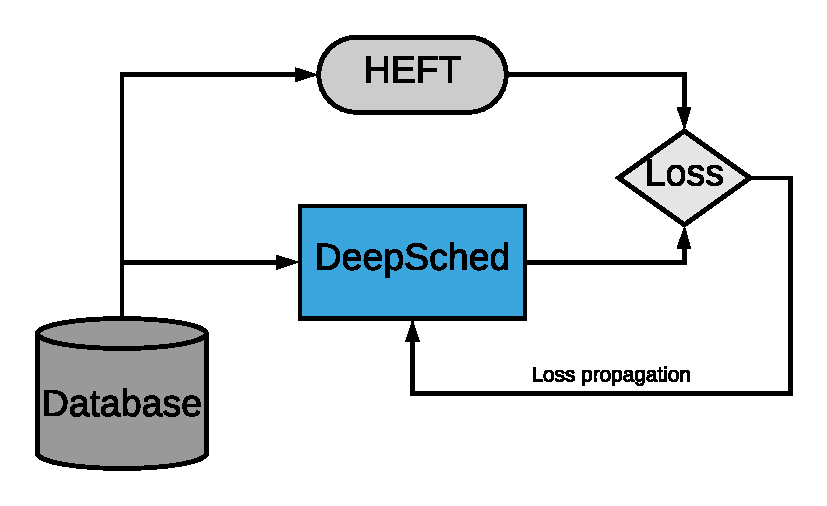
\includegraphics[width=0.45\textwidth]{diagrams/framework}
    \caption{The training framework of DeepSched network. A database of tasks and resources is provided for both network and HEFT. The loss of the network is measured based on HEFT produced schedule.}
    \label{fig:fw}
\end{figure}

Our evaluation methodology of the proposed network is based on comparison with two basic method. One of them is a heuristic method, which is \emph{Heterogeneous Earliest Time First} (HEFT) and the other is an approximate method, which is \emph{Genetic Algorithms} (GA). \\

The results are compared based on the execution time, as well as scheduling performance. For execution time, we measure the total time consumed by scheduling different number of tasks. For scheduling performance, we measure the total turnaround time for all scheduled tasks. Our network is supposed to achieve better execution time with similar performance to HEFT on previously seen data and slightly lower performance on unseen data. 

\subsection{Baseline}
HEFT, which is a heuristic method, is used as a comparison baseline and also to generate the training data, where the network approximates HEFT performance. GA solution, which is an approximate method, is only used as a comparison baseline. \\

\subsubsection{HEFT}
The basic architecture from the original paper \cite{993206} is used in a framework with the proposed neural network shown in Fig.\ref{fig:fw}. HEFT receives some data from a defined database of tasks and resources and produces the output schedule, which is used as labels for the network training data. This way the network can approximate the performance of the HEFT scheduling algorithm by learning to map the input tasks and resources to the schedule produced by HEFT on a large database. \\

\subsubsection{Genetic Algorithms}
The methodology from \cite{article2} is used to develop a genetic algorithm solution for heterogeneous systems. Extra parameters are added to the population to represent the different resources. Also, the execution time is expanded to be a value for each job running on a specific machine, instead of only one execution time value. The used fitness function is the average waiting time \ref{eq:ga}. Random initialization is used along with Crossover. The results of this method are compared to the output of the proposed network.

\subsection{Datasets}
A database of tasks and resources is adapted from \emph{Dataset for Task scheduling in Cloud using CLoudsim} \cite{px5b-b729-20}. The used database consists of $100000$ training samples represented as a list of tasks requires to be scheduled. Each training sample contains from $486$ to $84654$ tasks, arranged as a \emph{directed acyclic graph} (DAG) to represent the task dependencies and each task has an execution time for each specific processor. Also, the database contains $188$ resource instances (processors), on which the given tasks scheduled. The desired output of such data is to determine, for each task, the optimal processor to run on, the actual start time (AST) and the actual finish time (AFT). 

\subsection{Implementation Details}
Our proposed network consists of four main modules.

\subsubsection{Machine Encoder}
This module takes resource details as an input and learns a meaningful representation of them. It consists of one \emph{Conv1D} layer to extract the basic features of each processor, followed by one \emph{fully connected} layer to learn a compact representation of all processors, in order to be passed to the output modules. The common input features for each processor passed to this module are number of processor cores, core frequency and memory capacity. \\

\subsubsection{Task Encoder}
This module takes the time sequence of tasks required to be scheduled and learns a meaningful representation of them through time. \emph{Recurrent neural networks} are used to learn the desired temporal information of the tasks. The module consists of a single \emph{bidirectional gated recurrent unit} (GRU) \cite{chung2014empirical} layer to extract temporal features of each task, followed by one \emph{fully connected} layer to learn a compact representation of all tasks, in order to be passed to the output modules. The common input features for each task passed to this module are arrival time, burst (execution) time for each processor, task priority and memory utilization. \\

The outputs of the previous stages are fused with each other by stacking, in order to form one chunk of information, which is then passed to the two output modules. \\

\subsubsection{Classifier}
The target of this module is to select the optimal running processor for each task amongst the given set of processors. The input to this module is the stacked information of both resources and tasks. It consists of a single \emph{Conv1D} layer, which is used to select running processor for each single task in the form of one hot encoding of the length of resources number. \\

\subsubsection{Regressor}
The target of this module is to predict the actual start time and the actual finish time of each task on the scheduled processor. The input to this module is the stacked information of both resources and tasks. It consists of a single \emph{Conv1D} layer, which is used to regress the actual start and finish times for each task. 

\subsection{Training}
The network is trained on HEFT scheduling outputs. Cross-entropy is used as a classification loss and mean squared error (MSE) is used as a regression loss. The summation of the two losses \ref{eq:l} is used to train the network using gradient descent with \emph{Adam} optimizer and a learning rate of $1e$-$5$. The network is trained for $100$ epochs. The training takes around $1.5$ hours on \emph{Nvidia GTX} $1070$ and around $13$ hours on \emph{Nvidia GTX} $840m$, which is a relatively small time based on both \emph{GPUs} performance.

\subsection{Inference}
Inference is performed on the trained network using both seen and unseen data, in order to compare with both HEFT and genetic algorithms, based on time and performance.